%!TEX root =../../course-notes.tex
% ^ leave for LaTeXTools build functionality

\begin{applicationActivities}{2}{26}

\begin{fact}
By a geometric argument, one can show that the determinant of a matrix and its transpose are the same.    Thus, row operations behave like column operations.  In particular, we can use row reduction to compute determinants.
\end{fact}

\begin{fact}
We deduced yesterday that row operations change the determinant in the following way
\begin{enumerate}
\item Adding a multiple of one row to another does not change the determinant.
\item Multiplying a row by a scalar multiplies the determinant by the same amount.
\item Swapping two rows multiplies the determinant by $-1$.
\end{enumerate}
\end{fact}

\begin{activity}{10}
  Compute $\det \begin{bmatrix} 4 & 5 \\ 2 & 3 \end{bmatrix}$ by using row reduction.
\end{activity}

\begin{fact}
It is straightforward but slightly tedious to verify that $$\det \begin{bmatrix} a & b \\ c & d \end{bmatrix} = ad-bc.$$

You should feel free to use this formula to expedite your calculations.
\end{fact}


\begin{activity}{5}
  Which of the following is the same as $\det \begin{bmatrix} 3 & 1 & 0 \\  1 & 1 & 0 \\  0 & 0 & 1\end{bmatrix}$?
\begin{multicols}{2}
\begin{enumerate}[(a)]
\item $\det \begin{bmatrix} 3 & 1 \\ 1 & 1 \end{bmatrix}$
\item $\det \begin{bmatrix} 3 & 1 \\ 1 & 0 \end{bmatrix}$
\item $\det \begin{bmatrix} 3 & 1 \\ 0 & 1 \end{bmatrix}$
\item $\det \begin{bmatrix} 1 & 1 \\ 0 & 1 \end{bmatrix}$
\end{enumerate}

\begin{center}
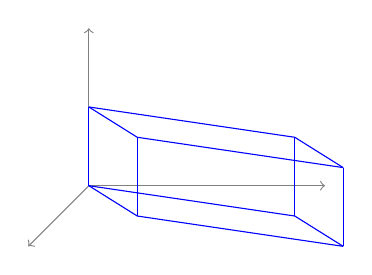
\begin{tikzpicture}
\draw[thin,gray,->] (0,0,0) -- (3,0,0);
\draw[thin,gray,->] (0,0,0) -- (0,2,0);
\draw[thin,gray,->] (0,0,0) -- (0,0,2);
%(y,z,x)

\draw[blue] (0,0,0) -- (0,1,0);
\draw[blue] (0,0,0) -- (1,0,1);
\draw[blue] (0,0,0) -- (3,0,1);
\draw[blue] (0,1,0) -- (1,1,1);
\draw[blue] (0,1,0) -- (3,1,1);
\draw[blue] (3,0,1) -- (4,0,2);
\draw[blue] (3,0,1) -- (3,1,1);
\draw[blue] (1,0,1) -- (4,0,2);
\draw[blue] (1,0,1) -- (1,1,1);
\draw[blue] (1,1,1) -- (4,1,2);
\draw[blue] (4,0,2) -- (4,1,2);
\draw[blue] (3,1,1) -- (4,1,2);
\end{tikzpicture}
\end{center}
\end{multicols}
\end{activity}

\begin{activity}{5}
  Which of the following is the same as $\det \begin{bmatrix} 3 & 1 & 0 \\  1 & 1 & 1 \\  0 & 0 & 1 \end{bmatrix}$?
  
\begin{multicols}{2}
\begin{enumerate}[(a)]
\item $\det \begin{bmatrix} 3 & 1 \\ 1 & 1 \end{bmatrix}$
\item $\det \begin{bmatrix} 3 & 1 \\ 1 & 0 \end{bmatrix}$
\item $\det \begin{bmatrix} 3 & 1 \\ 0 & 1 \end{bmatrix}$
\item $\det \begin{bmatrix} 1 & 1 \\ 0 & 1 \end{bmatrix}$
\end{enumerate}


\begin{center}
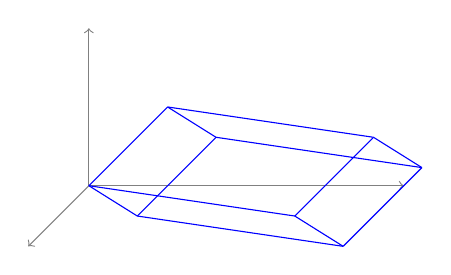
\begin{tikzpicture}
\draw[thin,gray,->] (0,0,0) -- (4,0,0);
\draw[thin,gray,->] (0,0,0) -- (0,2,0);
\draw[thin,gray,->] (0,0,0) -- (0,0,2);
%(y,z,x)

\draw[blue] (0,0,0) -- (1,1,0);
\draw[blue] (0,0,0) -- (1,0,1);
\draw[blue] (0,0,0) -- (3,0,1);
\draw[blue] (1,1,0) -- (2,1,1);
\draw[blue] (1,1,0) -- (4,1,1);
\draw[blue] (3,0,1) -- (4,0,2);
\draw[blue] (3,0,1) -- (4,1,1);
\draw[blue] (1,0,1) -- (4,0,2);
\draw[blue] (1,0,1) -- (2,1,1);
\draw[blue] (2,1,1) -- (5,1,2);
\draw[blue] (4,0,2) -- (5,1,2);
\draw[blue] (4,1,1) -- (5,1,2);
\end{tikzpicture}
\end{center}
\end{multicols}

{\em Hint: Use a row operation and the previous activity}
\end{activity}

\begin{observation}
If the $i$-th column or row is $\vec{e}_i$, then the determinant is the same as the determinant of the $(n-1) \times (n-1)$ submatrix with the $i$-th row and column removed.

\ \\

For example, 
$$\det \begin{bmatrix} 3 & 0 & -1 & 5 \\ 2 & 1 & 4 & 0 \\ -1 & 0 & 1 & 11 \\ 3 & 0 & 0 & 1 \end{bmatrix} = \det \begin{bmatrix} 3 & -1 & 5 \\ -1 & 1 & 11 \\ 3 & 0 & 1 \end{bmatrix}$$
\end{observation}

\begin{activity}{5}
  Which of the following is the same as $\det \begin{bmatrix} 2 & 0 & 1 \\  1 & 3 & 1 \\  0 & 0 & 2 \end{bmatrix}$?
  
\begin{multicols}{2}
\begin{enumerate}[(a)]
\item $3\begin{bmatrix} 2 & 1 \\ 0 & 2 \end{bmatrix}$
\item $3\begin{bmatrix} 2 & 0 \\ 1 & 3 \end{bmatrix}$
\item $3\begin{bmatrix} 2 & 1 \\ 1 & 1 \end{bmatrix}$
\item $3\begin{bmatrix} 3 & 1 \\ 0 & 2 \end{bmatrix}$
\end{enumerate}


\begin{center}
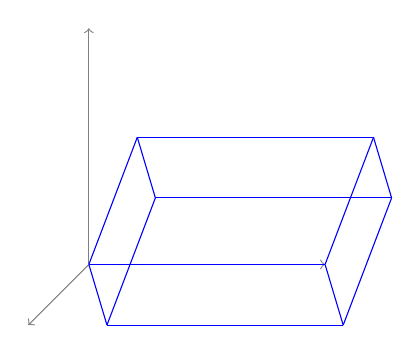
\begin{tikzpicture}
\draw[thin,gray,->] (0,0,0) -- (3,0,0);
\draw[thin,gray,->] (0,0,0) -- (0,3,0);
\draw[thin,gray,->] (0,0,0) -- (0,0,2);
%(y,z,x)

\draw[blue] (0,0,0) -- (1,0,2);
\draw[blue] (0,0,0) -- (1,2,1);
\draw[blue] (0,0,0) -- (3,0,0);
\draw[blue] (1,0,2) -- (2,2,3);
\draw[blue] (1,0,2) -- (4,0,2);
\draw[blue] (3,0,0) -- (4,0,2);
\draw[blue] (3,0,0) -- (4,2,1);
\draw[blue] (1,2,1) -- (2,2,3);
\draw[blue] (1,2,1) -- (4,2,1);
\draw[blue] (2,2,3) -- (5,2,3);
\draw[blue] (4,0,2) -- (5,2,3);
\draw[blue] (4,2,1) -- (5,2,3);
\end{tikzpicture}
\end{center}
\end{multicols}

\end{activity}


\begin{activity}{5}
  Compute $\det \begin{bmatrix} 0 & 3 & -2 \\ 1 & 5 & 12 \\ 0 & 2 & -1 \end{bmatrix}$.

  {\em Hint: Swap rows or columns to reduce to an easier problem}.
\end{activity}

\begin{activity}{10}
   Using the fact that $\begin{bmatrix} 2 \\ 1 \\ 0 \end{bmatrix} = \begin{bmatrix} 2 \\ 0 \\ 0 \end{bmatrix} + \begin{bmatrix} 0 \\ 1 \\ 0 \end{bmatrix}$, compute $\det \begin{bmatrix} 2 & 2 & 3 \\ 1 & -2 & -5 \\ 0 & 3 & 3 \end{bmatrix}$.
\end{activity}

\begin{activity}{10}
   Compute $\det \begin{bmatrix} 2 & 3 & 5  \\ 1 & 1 & 0  \\ -1 & 2 & -1 \end{bmatrix}$.
\end{activity}

\begin{activity}{10}
   Compute $\det \begin{bmatrix} 2 & 3 & 5 & 0 \\ 0 & 1 & -1 & 0 \\ 1 & 2 & 0 & 3 \\ -1 & -1 & 2 & 2 \end{bmatrix}$.
\end{activity}

\end{applicationActivities}
